\documentclass{bioinfo}
\usepackage{multirow}
\usepackage{booktabs}
\usepackage{amsmath}
\usepackage{color}
\copyrightyear{2014}
\pubyear{2014}

\newcommand{\comment}[1]{\textsl{\textcolor{Gray}{#1}}}
\newcommand{\fixme}[1]{\textsl{\textcolor{red}{FIXME: #1}}}
\newcommand{\emphref}[1]{\emph{\nameref{#1}}}

\begin{document}
\firstpage{1}

\title[Cross-study validation]{Dataset heterogeneity in the validation of prediction models across studies}
\author[Zhang \textit{et~al}]{Yuqing Zhang\,$^{1}$, Christoph Bernau\,$^{2,3}$, Giovanni Parmigiani\,$^{4,5}$ and Levi Waldron\,$^{6}$ \footnote{to whom correspondence should be addressed}}
\address{$^{1}$Boston University Bioinformatics Program, Boston, U.S.A\\
$^{2}$Leibniz Supercomputing Center, Garching, Germany\\
$^{3}$Department for Medical Informatics, Biometry and Epidemiology, Munich, Germany \\
$^{4}$Dana-Farber Cancer Institute, Boston, U.S.A\\
$^{5}$Harvard School of Public Health, Boston, U.S.A\\
$^{6}$School of Urban Public Health at Hunter College, City University of New York, New York, U.S.A}

\history{Received on XXXXX; revised on XXXXX; accepted on XXXXX}

\editor{Associate Editor: XXXXXXX}

\maketitle

\begin{abstract}

  \section{Motivation:} Cross-study validation (CSV) of prediction
  models is an alternative to traditional cross-validation (CV) in
  research domains where multiple comparable datasets are
  available. Although many studies have noted potential sources of
  heterogeneity in genomic studies, to our knowledge none have
  systematically investigated their intertwined impacts on prediction
  accuracy.

  \section{Methods:} %We employ a hybrid parametric/non-parametric
%  bootstrap method to generate realistic simulations based on 
%  publicly available microarray datasets. Two collections of studies, one for estrogen
%  receptor-positive breast cancer with disease and metastasis-free
%  survival outcome and one for ovarian cancer, are used. With two prognostic algorithms, 
  We employ a hybrid parametric/non-parametric bootstrap 
  method to generate realistic simulations based on 
  publicly available breast and ovarian cancer microarray datasets,
  where two predictive models are validated within and
  across studies.
  Three types of heterogeneity between studies are
  manipulated and studied: 1) imbalances in the prevalence of
  clinical and pathological covariates, 2) differences in gene covariance that could be caused
  by batch, platform, or tumor purity effects, and 3) differences in
  the "true" model that associates gene expression and clinical factors to outcome,
  including model coefficients and baseline hazard. We assessed model
  accuracy by Concordance Index (C-Index) within and across studies
  while altering these factors and the combination of all of them.

   \section{Results:} Lower accuracy is seen between than within
  studies, and the difference cannot be explained by heterogeneity in
  the available clinical covariates or by differences in gene
  covariance.  %Both corrections, in combination with 
  Forcing identical
  generative models nearly eliminates the
  within/across study difference for both cancer types. 
  These results suggest that the most
  easily identifiable sources of study heterogeneity may not be the
  primary ones determining the ability to translate prediction models
  across studies.

  \section{Availability:} The simulation methodology is implemented as
  the \emph{simulatorZ: Simulator for Collections of Independent
    Genomic Datasets} Bioconductor package\\
  (http://bioconductor.org/packages/release/bioc/html/simulatorZ.html).
\end{abstract}

\section{Introduction}
Quantification of heterogeneity between studies and its impact on
validation of decision models is important across a wide range of
applications.  A special issue of Briefings in Bioinformatics
(Validation in Bioinformatics and Molecular Medicine, May 2011)
emphasized that independent validation of genomic classifiers is rare
\citep{Castaldi2011-dl}, and that difficulty with external validation
and study heterogeneity is common not only in microarray studies but
extends to GWAS studies \citep{Konig2011-el}.  External validation is
critical in any research domain affected by heterogeneous samples,
sample selection bias, or technical batch effects.  However it has
proven especially difficult for classifiers and subtypes identified
from gene expression data.  Patient populations can be heterogeneous in their
exposures, geography, race/ethnicity, and socioeconomic status, and
these differences could manifest as biologically distinct forms of
disease that vary systematically between studies.  Adding to the
potential for study bias, clinical tissue specimens are costly and
difficult to collect, and time-consuming to connect with clinical
follow-up.  What statisticians call ``samples of convenience'' are the
norm in translational genomics research \citep{Simon2009}, even though
convenience hardly describes the process of collecting and assaying
clinical specimens.  Methods for correction of validation accuracy
estimation in biased samples have been proposed \citep{Cortes2008},
but only when the unbiased distribution of covariates is known. In the
practice of developing genomic prediction models, all potential sources of
heterogeneity are likely not even known.  Finally, batch effects
\citep{Leek2010} and platform effects impact on reproducibility across
studies, but sources of batch variation often are not known.  In spite
of these challenges, we expect clinically-relevant genomic findings to
be reproducible at hospitals around the world, suggesting robustness
in the presence of some heterogeneity.  The ``molecular portraits'' of
breast cancer, for example, have been broadly reproduced across
platforms and centers \citep{Hu2006}.  Heterogeneity between clinical
studies cannot be avoided, but we propose that the impact even of
still-unidentified sources of heterogeneity can be accounted for and
quantified if independent studies are available.

Previous studies have shown that accuracy estimates of genomic
prediction models based on independent validation are inferior to
cross-validation estimates \citep{Castaldi2011-dl, Bernau2014}, but
did not identify the sources of heterogeneity responsible.  A standard
approach is to remove as many sources of heterogeneity as possible,
such as \citet{Waldron2014} and \citet{Riester2014}, which limited
meta-analyses to late-stage, high-grade, serous ovarian
cancer. Similarly, recommendations for the replication of genome-wide
association studies include studying a "similar" population.
However in many cases it is unclear what measures of study similarity are
important, and unnecessarily restrictive inclusion criteria have costs
in reduced sample size and loss of generality of findings.
Thus the question arises of which sources of heterogeneity do in fact
impact the accuracy of cross-study prediction, and how these can be
determined from the data when independent studies are available.

We compare within and across-study validation of omics-based prediction models
using simulations which are generated from two collections of publicly
available experimental datasets, for estrogen-receptor positive breast cancer 
and for late-stage, high-grade ovarian cancer. %We compare within and across-study validation of microarray-based
%prognostic models of estrogen receptor-positive breast cancer, using
%simulations that mimic the propoerties of a compendium of publicly
%available, independent experimental datasets.
We investigate the impact of three possible types of heterogeneity on cross-study
validation performance: changes in prevalence of known clinical and
pathologic factors, changes in gene expression covariance structure
for example due to batch or platform effects, and changes in the true
models associating gene expression and clinical factors with outcome.  
These sources of heterogeneity are manipulated and equalized in turn, 
while comparing within- to across-study validation of risk scores for 
%disease and metastasis-free 
survival. The methodology of this study can be applied to
investigating the effects of study heterogeneity on model validation
in any scenario where multiple independent but comparable datasets are available.


% Unlike in traditional
% cross-validation, the prevalence of clinical covariates of known
% prognostic importance, such as tumor stage, can differ greatly between
% studies. Combination of multiple datasets in cross-study validation
% also introduces a new question whether genes selected possess
% reliability. Integrative Correlation \citep{Garrett-Mayer2008} is a
% measurement suitable for assessing the genes involved. Finally, in the
% simulation, if we fit the parametric model separately for each
% independent set, differences in the true model of every simulated sets
% is another potential source explain the reduction in risk score
% performance across studies versus within studies.

\section{Methods}

%  \citet{Bernau2014} introduced a systematic approach for synthesizing a
%  group of independent microarray datasets with survival outcome for
%  cross-study assessment of prediction algorithms. The simulation
%  procedure, which involves a combination of non-parametric bootstrap
%  (resampling of studies and individual patients) and parametric bootstrap 
%  (a "true" generative model for simulating realistic survival times and censoring status based on
%  the "original" dataset), will be summarized here. We implement this
%  simulation procedure as the \emph{survHD} Bioconductor package, and
%  provide all additional codes for reproducing
%  the results of this paper at
%  \\ https://bitbucket.org/zhangyuqing/datasetheterogeneity.
%  \subsection{The \emph{simulatorZ} Bioconductor package}

  \citet{Bernau2014} introduced a systematic approach for synthesizing a
  group of independent microarray datasets with survival outcome for
  cross-study assessment of prediction algorithms. %, to replace or supplement 
  %conventional cross-validation when evaluating prediction models in 
  %independent datasets. 
  This approach was illustrated with estrogen-receptor 
  positive breast cancer microarray datasets, and performance statistics of cross-study 
  and conventional cross-validation were compared.
  
  In the current work, we review the simulation procedure in the following sections, 
  which involves a 3-step bootstrap method. We implemented this simulation approach 
  in the \emph{simulatorZ} package available on Bioconductor. Scripts for reproducing
  the results of this paper are stored and documented at
  \\ https://bitbucket.org/zhangyuqing/datasetheterogeneity. 
  
  \subsection{Datasets}

  The simulations were performed on two collections of cancer studies, with the first group
   being the curated breast cancer datasets used in the work of \citet{Bernau2014}.
  This compendium of microarray datasets was originally published by \citet{Haibe-Kains2012},
  with censored disease and metastasis-free survival (DMFS) response 
  and estrogen-receptor positive breast cancer individuals. Datasets originating
  from more than one study were separated into their base sets. 10 base
  sets involved in the previous study were considered for inclusion:
  CAL, MAINZ, MSK, EXPO, TRANSBIG, UNT, VDX,
  MDA4, SUPERTAM\_HGU133A and SUPERTAM\_HGU133PLUS2 (the latter four
  were referred as VDX3, MDA5, and TAM by \citet{Bernau2014}). MDA4 and EXPO were
  excluded for the lack of the DMFS information. As illustrated in \citet{Haibe-Kains2012}, 
  we linearly scaled the gene expressions based on the 2.5\% and 97.5\% quantiles. Among genes
  shared across the remaining 8 datasets, 40\% with high variances 
  were selected, which led to 5307 genes. 
  Samples from SUPERTAM\_HGU133A duplicated in VDX were removed. 
  Missing expression values were imputed by the K-nearest neighbors approach \citep{KNN}.

  Available clinical and pathological covariates in these datasets include PGR and HER2 expressing status, histological
  grade, tumor size, nodal status, and patient age at diagnosis. Age and tumor size were
  dichotomized at 50 years and 2cm, respectively
  \citep{Haibe-Kains2012}, and grade was maintained as three levels
  (low/medium/high) as in the original datasets. 
% Unnecessary detail I think: Grade is dichotomized into two 0-1 variables when obtaining the true
%  coefficients(one for high vs. medium + low, one for medium vs. high + low).
%  When balancing the prevalence of grade, it is remained as the three-level
%  covariate in the original datasets.
PGR, nodal status and HER2 were available in 5, 4, and 2
  datasets respectively. Thus only tumor size, grade and patient age 
  were considered as available clinical factors. 
     %so for primary simulations we considered only
  %tumor size and grade, and patient age to avoid losing
  %additional datasets. We then considered PGR alone in a separate
  %simulation study. 
  Patients missing any of these three 
  clinical factors, or with zero follow-up, were
  excluded. Supplementary Table 1 shows detailed availability of covariate information in each data
  set.
  
  Finally, datasets with fewer than 40 individuals were
  removed. The remaining 7 data sets are referred to as the
  "original datasets" (Table \ref{table-datasets}), with 1021 patients combined. 
  Synthesized Hazard Ratios (HR) of the tumor size, grade and patient age are 1.96, 1.65 and 1.2 
  (Supplementary Table 2). This is consistent with commonly
  used prognostic factors for primary breast cancer such as the
  Nottingham Prognostic Index \citep{haybittle1982prognostic}, 
  showing that the dichotomized tumor size
  and grade are prognostic. 
     

\begin{table*}[!t]
    \begin{tabular*}{1\textwidth}{@{\extracolsep{\fill}}lllllllll}
      NO. & Name & \#patients & \%$>$2cm &  \%high-grade & \%medium-grade & \%low-grade & \%$>$50yrs  &reference\\
      \hline
      1 & CAL & 68 & 63.2  & 57.4 & 35.3 & 7.4 & 61.8 & \citet{chin2006genomic} \\ %Chin et al. (2006)\\
       \hline
      2 & MNZ & 162 & 40.7  & 9.9 & 73.5 & 16.7 & 76.5 & \citet{schmidt2008humoral} \\ %Schmidt et al. (2008) \\
      \hline
      3 & TAM1 & 317 & 58.0  & 18.3 & 58.4 & 23.3 & 91.2 & \citet{foekens2006multicenter}\\%Foekens et al. (2006)\\
       \hline
      4 & TAM2 & 128 & 53.1  & 31.3 & 44.5 & 24.2 & 93.0 & \citet{symmans2010genomic}\\%Symmans et al. (2010)\\
       \hline
      5 & TRB  & 132 & 43.2  & 26.5 & 51.5 & 22.0 & 29.5 & \citet{desmedt2007strong} \\%Desmedt et al. (2007)\\
       \hline
      6 & UNT  & 72 & 38.9  & 16.7& 43.1 & 40.3 & 59.7 & \citet{sotiriou2006gene} \\%Sotiriou et al. (2006)\\
       \hline
      7 & VDX  & 142 & 2.8 & 71.8 & 25.4 & 2.8 & 57.7 & \citet{minn2007lung} \\%Minn et al. (2007)\\
       \hline
      \quad & overall & 1021 & 44.1 & 29.6 & 50.9 & 19.5 & 72.3 &  \quad \\
      \hline
    \end{tabular*}
    \caption{\textbf{Breast cancer microarray datasets divided into
        base sets as used in this study}. Percentages are rounded to the nearest tenth. Datasets
      acronyms: CAL = University of California,
      San Francisco and the California Pacific Medical Center (United
      States), MNZ = Mainz hospital (Germany), TAM1 and TAM2 represents
      SUPERTAM\_HGU133A and SUPERTAM\_HGU133PLUS2, which are provided by \citet{Haibe-Kains2012}, 
      TRB = TransBIG consortium dataset (Europe), UNT = the cohort of
      untreated patients from the Oxford Radcliffe Hospital (United
      Kingdom), VDX = Veridex (the Netherlands). Column lables:
      \#patients = the number of patients after cleaning. \%$>$2cm =
      percentage of patients in cleaned datasets with tumor size
      larger than 2cm. \%low, medium and high-grade refer to percentage
      of patients with high, intermediate and low level of histological grade
      respectively. \%$>$50yrs = percentage of patients older than 50 years.}
    \label{table-datasets}
  \end{table*}
  
  The other collection of ovarian cancer microarray datasets was published in
  \citet{Ganzfried2013} and made available through the \emph{curatedOvarianData} 
  Bioconductor package. To select a group of studies for simulation, 
  we filtered datasets with at least 1000 genes, 40 individuals and 15 events. Batch effect was
  adjusted within each data set when the batch information was available, 
  and the expression values were standardized with z-score scaling.
  Missing values in the expression matrices 
  were imputed by the K-nearest neighbors approach \citep{KNN}. We then took the overlapped 
  genes across all studies, and removed all genes with a standard deviation below 
  the 60\% quantile in every selected dataset, which resulted in 7484 gene features.
 
  Patients with late-stage, high-grade cancer were included. 
  The datasets contain patient age and debulking as available 
  clinical covariates. Samples with missing values for these covariates or the outcome were removed. The patient age was dichotomized at 70 years. Distributions 
  of these covariates are summarized in Table \ref{table-datasets-ovarian}. Synthesized Hazard Ratios 
  of these covariates are 1.84 (age) and 1.48 (debulking), 
  as shown in Supplementary Table 3. Forest plots of HR for 
  each covariate in these two collections of data
  are provided (Supplementary Figure 2). After cleaning, 5 microarray datasets were selected as the "original datasets" for ovarian cancer, with 935 patients in the collection.
  

  \subsection{The \emph{simulatorZ} Bioconductor package}
 
 \begin{table*}[!t]
    \begin{tabular*}{1\textwidth}{@{\extracolsep{\fill}}llllll}
      NO. & Name & \#patients & \%$>$70yrs & \%suboptimal & reference\\
      \hline
      1 & E.MTAB.386 & 124 & 29.8 & 22.6  &  \citet{bentink2012angiogenic} \\
       \hline
       2 & GSE26712 & 182 & 24.7 & 51.1 & \citet{bonome2008gene} \\
      %\hline
       %3 & GSE30161 & 50 & 30 & 46 & 58 & 100 &  \citet{ferriss2012multi}\\
       \hline
       3 & GSE49997 & 136 & 14.7 & 31.6 & \citet{pils2012validating} \\
       \hline
       4 & GSE9891 & 124 & 19.4 & 42.7  & \citet{tothill2008novel} \\
       %\hline
       %6 & TCGA.RNASeqV2 & 225 & 19.1 & 74.7  & \citet{cancer2011integrated} \\
       \hline
       5 & TCGA & 369 & 23.3 & 27.6 & \citet{cancer2011integrated} \\
       \hline
      \quad & overall & 935 & 22.7 &  34.1 & \\
      \hline
    \end{tabular*}
    \caption{\textbf{Ovarian cancer microarray datasets}. Column lables:
      \#patients = the number of patients after cleaning. \%$>$70yrs = percentage 
      of patients older than 70 years. \%suboptimal =
      percentage of patients in cleaned datasets with suboptimally debulked tumors, as opposed to the optimally debulked ones.}%
      %\%high-grade = percentage of patients with high level of histological grade. 
      %\%late-stage = percentage of patients in late-stage ovarian cancer.}
    \label{table-datasets-ovarian}
  \end{table*}
  
  The \emph{simulatorZ} Bioconductor package was developed to
  create a collection of independent genomic datasets with
  realistic properties and time-to-event outcome generated from a
  known risk model. It also implements the M\'{a}s-o-menos algorithm
  \citep{Zhao2014} and provides basic facilities for 
  cross-validation and cross-study validation of prognostic models.
  It supports \emph{ExpressionSet} objects to simulate
  identifier-based data such as from microarray, and
  \emph{SummarizedExperiment} objects to simulate genomic range-based
  data such as from DNA and RNA sequencing.

    \subsubsection{Simulation Approach}
    The simulation procedure is in three steps. The first is a non-parametric
    bootstrap at dataset level, in which datasets are sampled with
    replacement from the list of original datasets. This
    estimates variability due to sampling of studies from a
    ``super-population'' of studies \citep{Hartley1975-bj}.  The
    second step is another
    non-parametric bootstrap resampling at the patient
    level, where a number of observations are sampled with replacement from
    each dataset selected in step 1.
    In the final step, a proportional hazards model is fit to the \emph{original} datasets, then used to
    simulate time-to-event on the simulated sets (parametric
    bootstrap):

    \begin{equation}\label{coxfunction}
      M^{j}_{true} : \lambda^{j}(t|x) = \lambda^{j}_{0}(t) * \exp(\beta_{j}^{T}x)
    \end{equation}

    $M^{j}_{true}$ is the true PH model for the j-th data set,
    whose hazard function is expressed with $\lambda^{j}(t|x)$,
    with $x$ as covariates. $\lambda^{j}_{0}(t)$ is the baseline
    hazard function for this set. $\beta$ represents the regression
    coefficients.

    The generative model in step 3 combines the truncated inversion
    method of \citet{Bender2005}, the Nelson-Aalen estimator
    \citep{Nelson1969,Nelson1972,Aalen1978}
    for cumulative hazard functions, and the \emph{CoxBoost} method of
    generating best-fit linear risk scores
    \citep{Binder2008}. Detailed methods can be found in the references;
    here we briefly illustrate the work flow. We first
    use \emph{CoxBoost} to obtain coefficients of linear predictors
    fitted to the original base datasets, using the genes plus the 
    clinical covariates, such as
    tumor size, debulking, histological grade and patient age, as predictors.
    The prognostic covariates were included to be mandatory unpenalized.
    We also obtained Nelson-Aalen estimator of baseline cumulative survival and
    censoring hazard, which, together with the \emph{CoxBoost}
    coefficients and equation \ref{coxfunction}, defined the "true"
    models of disease-free survival for each dataset.  Finally, we have:

    \begin{equation}\label{uniformrv}
      U = S(T) = \exp[-H_{0}(T) * \exp(\beta^{T}x)] \thicksim Uni[0,1]
    \end{equation}

    $H_{0}$ is the baseline cumulative hazard for the lifetime random variable $T$. $S$ donates the survival function. We sample two independent, uniformly distributed
    variables $u1$ and $u2$, then simulate the survival ($T$) and censoring ($C$)
    time, with

    \begin{equation}\label{survivaltime}
      T = H_{surv_{0}}^{-1} [ - \log(u1) * \exp(-\beta^{T}x)]
    \end{equation}
    \begin{equation}\label{censoringtime}
      C = H_{cens_{0}}^{-1} [ - \log(u2) * \exp(-\beta^{T}x)]
    \end{equation}

    $H_{surv_{0}}^{-1}$ and $H_{cens_{0}}^{-1}$ are the inverses
    of baseline cumulative survival and censoring hazard, respectively.  These
    are inverted by finding
    the point on the time line such that the values calculated by
    $- \log(u) * \exp(- \beta^{T}x)$ are closest in absolute value to the
    cumulative hazards. The simulated survival response is the smaller one between
    $T$ and $C$. This completes the simulation of datasets.

	The M\'{a}s-o-menos algorithm \citep{Zhao2014} and ridge 
	regression \citep{hoerl1970ridge} were chosen as
    examples of predictive models to generate risk scores on the simulated datasets. 
    We repeated 100 simulations and model validations 
    for each of the three dataset / algorithm combinations, 
    which are breast cancer data with M\'{a}s-o-menos and ridge regression methods, 
    and ovarian cancer with the M\'{a}s-o-menos algorithm.
    
    In each of 100 iterations, we simulated a list of independent datasets of
    sample size $n=150$ using the "original sets" and this 3-step bootstrap approach.  We
    then generated a matrix of C-indices as described by
    \citet{Bernau2014}, using predictive algorithms. %We noted that
   % popular alternatives to the M\'{a}s-o-menos algorithm, such as
   % Ridge Regression, produced consistent results. 
    Cross study validation (CSV) performance was summarized by the
    simple average of C-statistics for training and validation across
    all pairs of independent studies (off-diagonal elements of the
    matrix), and performance of the 4-fold cross validation (CV) was summarized by the average
    of the diagonal elements \citep{Bernau2014}. The process was
    repeated while altering potential sources of across-study
    heterogeneity, as described in the next three subsections of
    Methods. The workflow of methods are summarized in Figure \ref{scheme}.

\begin{figure*}[htp]
    \centering
    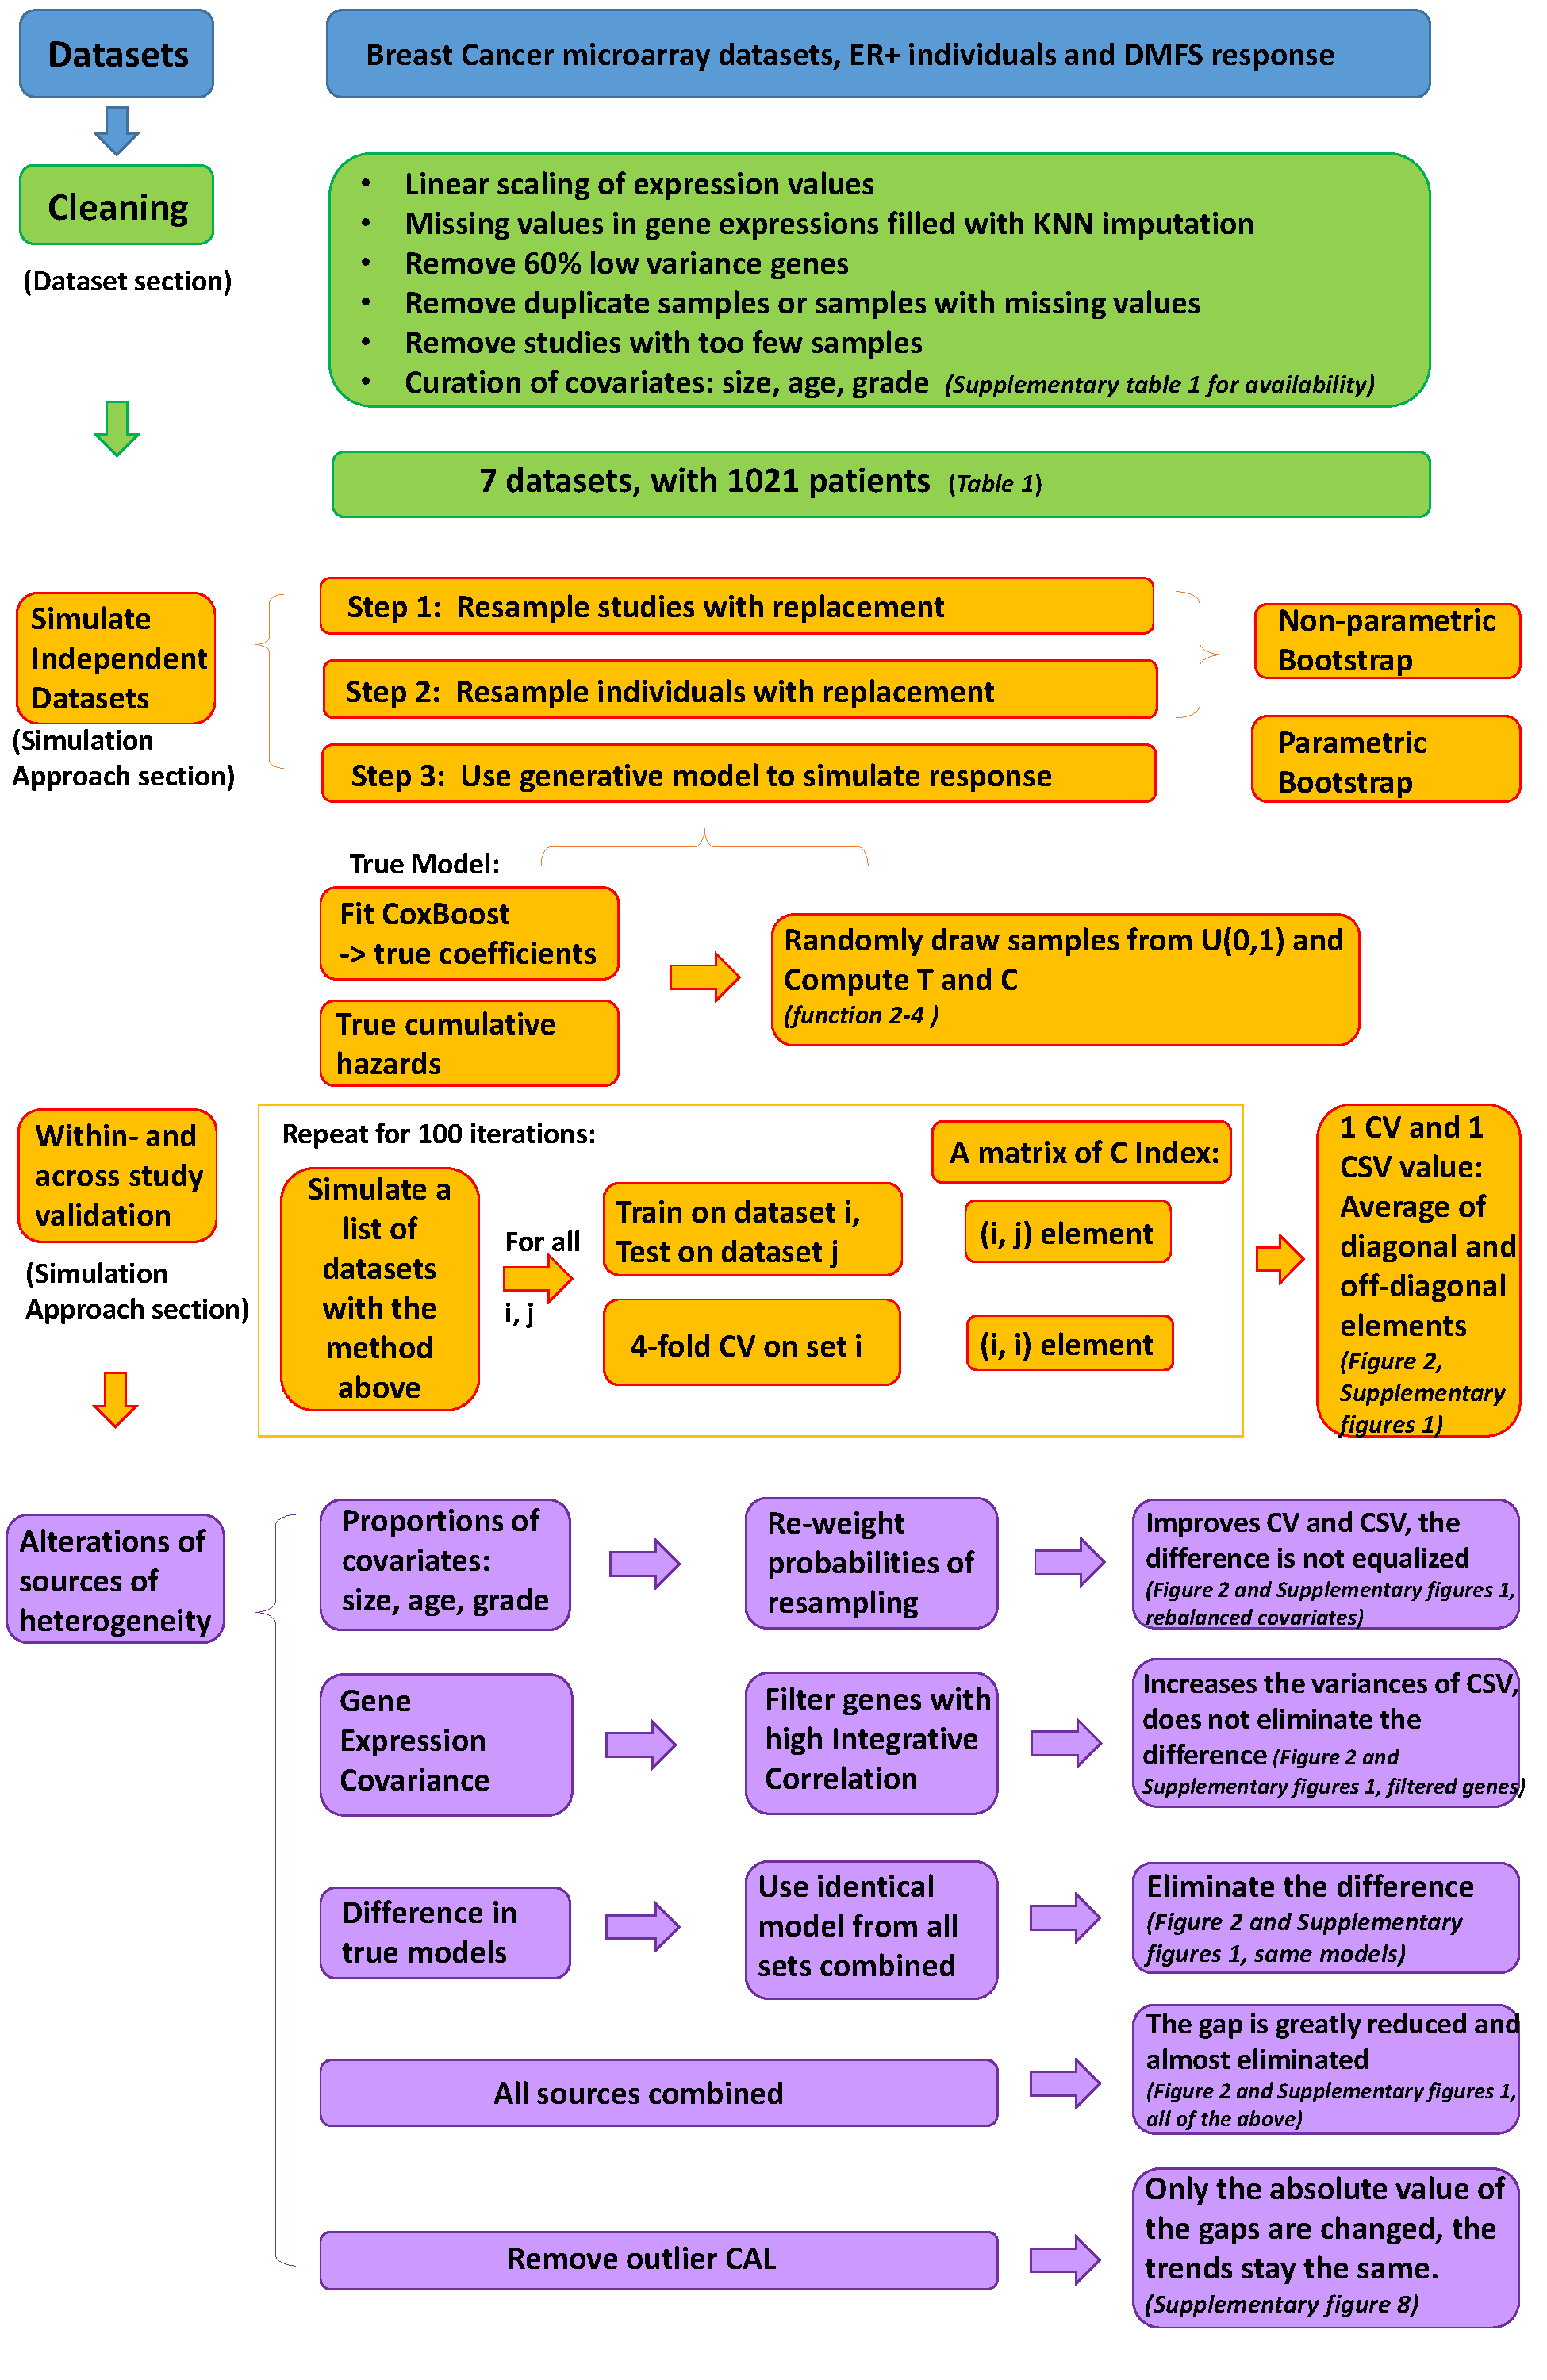
\includegraphics[width=12.5cm]{schema_update_new.pdf}\\
    \caption{\textbf{A schema of our study}. Methods and major results for breast cancer are summarized in this flow chart. Equivalent methods were employed for ovarian cancer. }
    \label{scheme}
  \end{figure*}

  \subsection{Clinical Covariates}

  The proportions of covariates such as tumor size, grade, debulking and of young and old
  patients were balanced so that on average, each simulated study would have
  proportions equal to the overall proportions.  To
  balance on multiple covariates, we re-weighted individual bootstrap
  sampling probabilities of each patient to result in identical joint
  probability distributions of the clinical / pathologic covariates
  across datasets.  Re-weighting of the sampling probabilities, rather
  than enforcing strict equality of covariate proportions, reflects
  the reality that these proportions are subject to sampling
  variation.

  	\subsubsection{Mixed-Effect Models}
  	To quantify the impact of balancing population attributes to the C-statistics
  	in cross-study validation, we built a linear model for each of the clinical factors, treating the
  	changes in covariate distribution in both the training and the test set 
  	as fixed effects, with random slopes varying across 100 simulations. 
  	Such a linear model is formulated as
  	
  	\begin{equation}\label{linmod}
      \Delta C \sim \Delta cov(train) + \Delta cov(test) + interaction
    \end{equation}
    
    For instance, the linear model for patient age at diagnosis is
  
%  	\begin{align}\label{linmod-exp}
%  	\begin{split}
%      \Delta C \sim & \Delta \%old(train) + \Delta \%old(test) + \\
%                    & \Delta \%old(train):\Delta \%old(test)
%    \end{split}
%    \end{align}
	
	\begin{equation}
		\footnotesize
		\Delta C \sim \Delta \%old(train) + \Delta \%old(test) + \Delta \%old(train):\Delta \%old(test)
	\end{equation}	
	
	where $\Delta$ represents the differences of values computed on
	simulations with balanced covariates compared to those with the unbalanced ones. $C$ stands for the cross-study validation score 
	calculated from the performance matrices. $\%old(train)$ and $\%old(test)$ are the percentage 
	of old patients in the training and the test set. The last term is the interaction 
	between the two main effects. For each dataset / algorithm combination, we 
	used the off-diagonal elements in 100 matrices of C-indices to form the design matrix. All terms 
	in the linear model are regarded as fixed effects with random slopes, 
	which avoids treating observations as independent within each simulation. %To address the overfitting issues,  avoid treating the multiple simulations as pseudo-replication
	%we simplified the model for some of the covariates by removing the interaction term 
	%according to the data.
	
  \subsection{Expression Covariance}
  To mitigate the potential impact of heterogeneity between gene
  expression levels in different datasets, we used only genes with
  high Integrative Correlation \citep{Parmigiani2004, Garrett-Mayer2008} assessed
  between every dataset pair. Briefly, we first calculated the Pearson
  correlation matrix of each gene expression matrix. For each pair of
  datasets, the Pearson correlation of the $k$-th rows of the two
  correlation matrices is the Integrative Correlation of gene $k$. 
  We did a grid search for the threshold of the Integrative Correlation,
  such that around 1000 genes with
  the highest Integrative Correlation scores between every pair
  of \emph{original} datasets were included. We also used arbitrary cut-offs 0.4 for 
  breast cancer and 0.2 for ovarian cancer, as comparison.

  \subsection{True Models}
  We equalized the ``true models'' of each dataset separately in terms
  of coefficients of the linear risk score for each dataset, and
  the baseline hazard function.  The common true model was fitted using
  all original datasets combined into a single large dataset.  However
  this model achieved much lower within-study performance than the
  baseline simulation. To increase CV to the same average C-Index as achieved without
  equalized coefficients, we multiplied all equalized coefficients
  by a constant factor of 1.6 in all dataset / algorithm combinations, that resulted 
  in CV performance similar
  to the baseline simulation.% (compare panels \emph{a} and \emph{d} in figure
%  \ref{boxplots}).


  

  \begin{figure*}[htp]
     \centering
     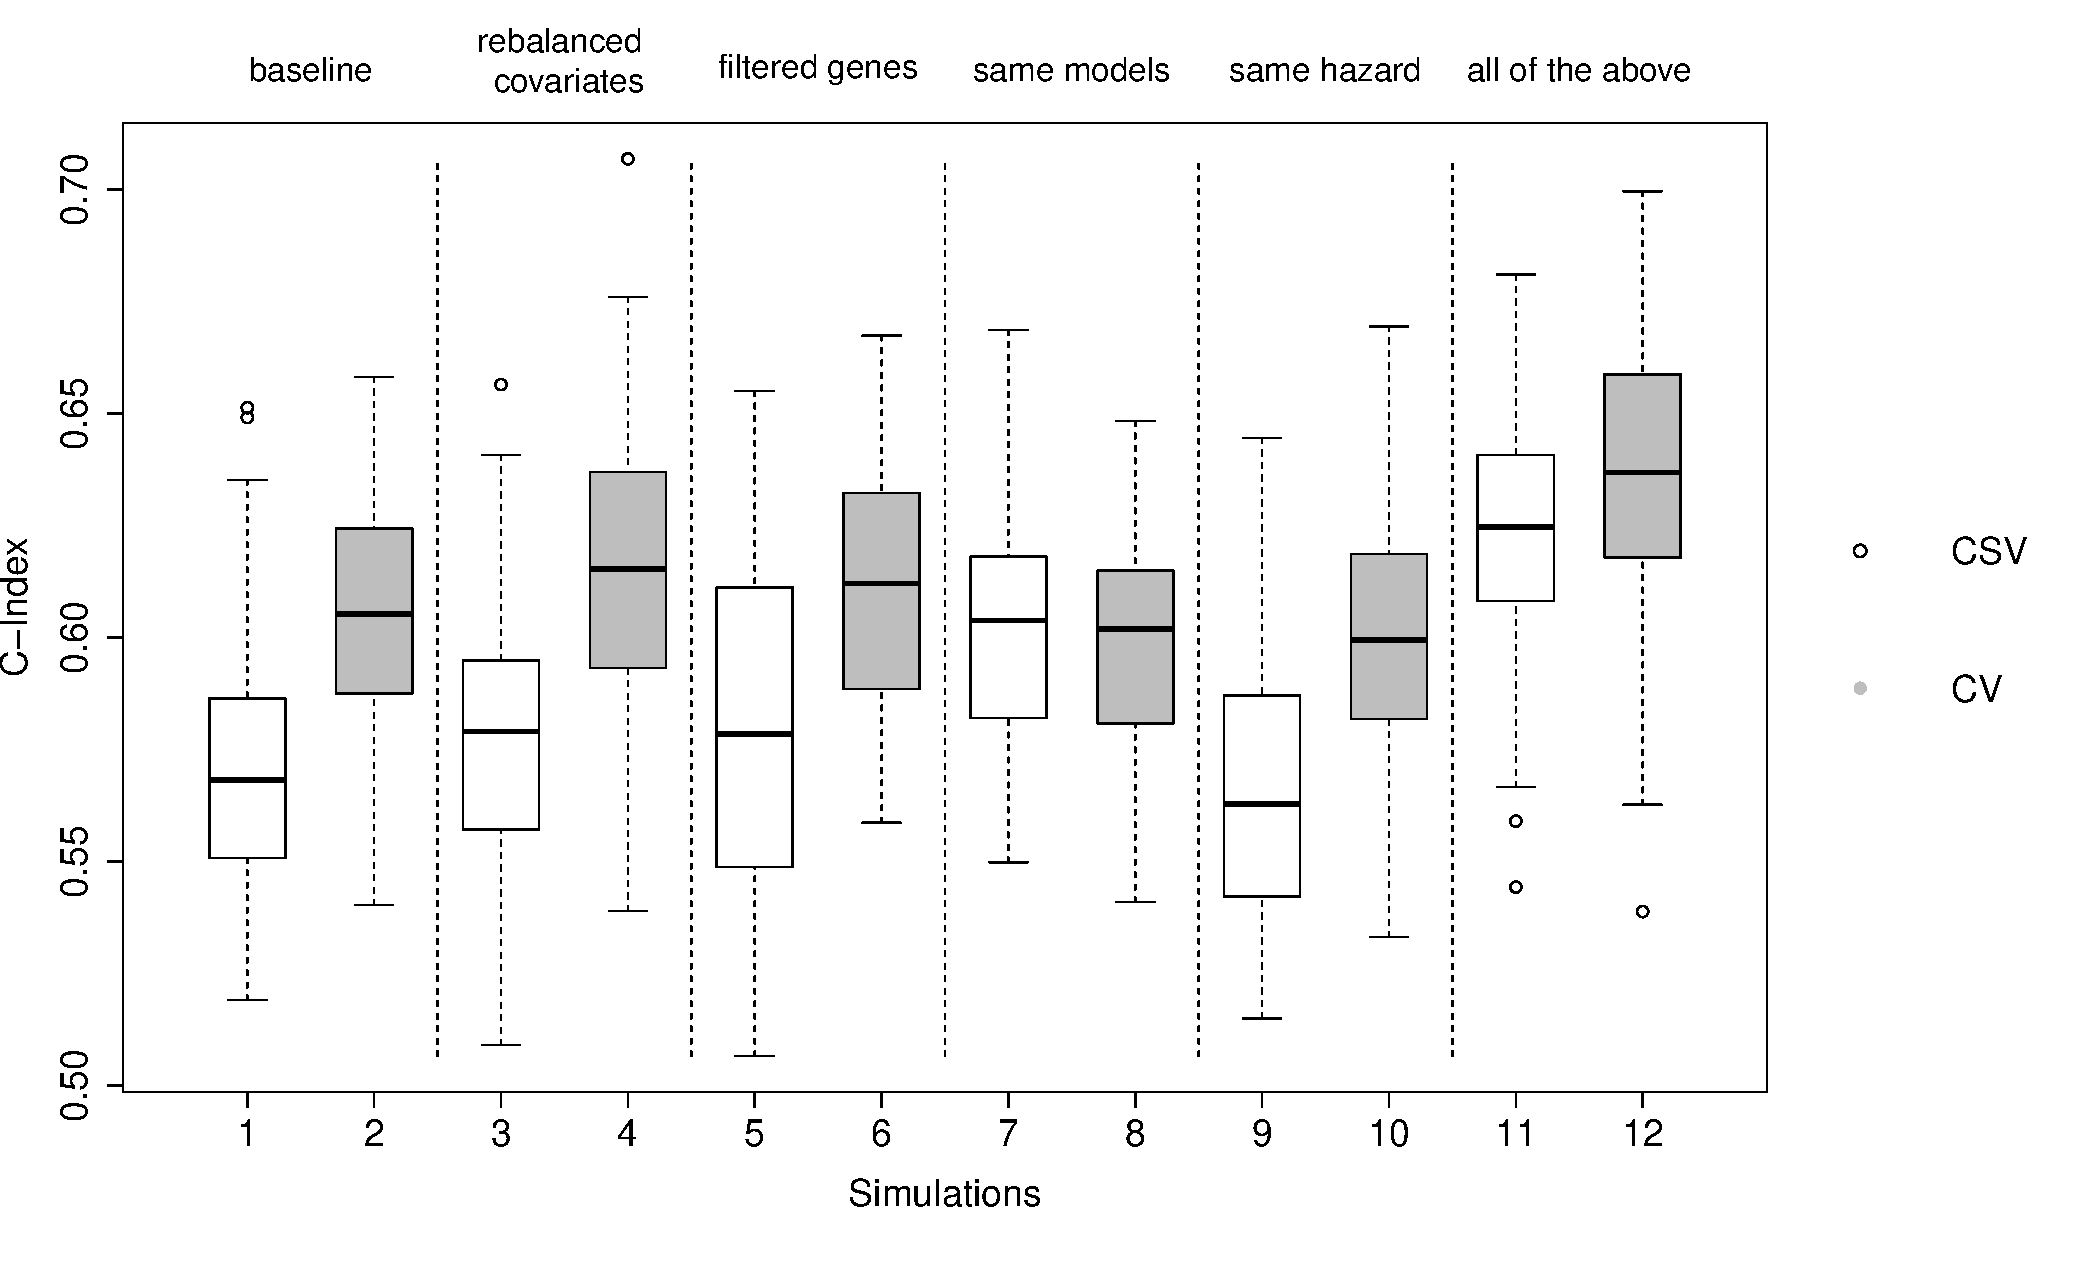
\includegraphics[width=16cm]{boxplot_breast_masomenos_withnames.pdf}
     \caption{\textbf{Simulation results comparing performances of CV and CSV for training M\'{a}s-o-menos on breast cancer data.} Panel "baseline" is a baseline scenario without considering any source of heterogeneity. In "rebalanced covariates", we change the re-sampling probability to coalesce with the distribution of covariates. The differences between CV and CSV are not eliminated. Panel "filtered genes" considers around 1000 genes with high Integrative Correlation, which increases the variance of CSV, but does not explain the difference as well. "Same models" shows great change using the same true model, i.e., the same coefficients from \emph{CoxBoost} and cumulative hazard in simulation. %C-indices of CV is even mildly lower than CSV, which could result from that size of training set in CV is smaller than that in CSV. 
         Panel "same hazard" separates the "true" model and uses the same cumulative hazard, but different coefficients for simulation. The fact that CSV drops back suggests that true coefficients is mainly responsible for the change in "same models". In "all of the above", all three heterogeneity sources were equalized. A gap is reintroduced in between CV and CSV compared to using only identical models, but the difference is greatly reduced compared to the baseline simulation. This figure is our major result which shows that the same true model can largely mitigate and even remove the differences between CSV and CV, while the other two factors cannot explain the performance drop of CSV. Results for the other two dataset / algorithm combinations are displayed in Supplementary Figure 1.}
     \label{boxplot_breast_masomenos}
  \end{figure*}

\section{Results}

\begin{table}[htbp]
  \centering
    \begin{tabular}{llll}
    \toprule
    \multicolumn{4}{c}{Breast Cancer} \\
    \midrule
          &       & M\'{a}s-o-menos & Ridge Regression \\
    \hline
    age   & train & 0.026 * & 0.012 \\
          &       & (0.011) & (0.010) \\
          & test  & 0.023 * & 0.027 * \\
          &       & (0.011) & (0.012) \\
          & interaction & -0.086 . & 0.008 \\
          &       & (0.049) & (0.046) \\
    size  & train & -0.036 ** & -0.003 \\
          &       & (0.013) & (0.019) \\
          & test  & -0.024 . & 0.022 \\
          &       & (0.014) & (0.023) \\
          & interaction & -0.119 & -0.173 \\
          &       & (0.108) & (0.146) \\
    grade & train (high) & -0.039 * & -0.026 \\
          &       & (0.018) & (0.020) \\
          & test (high) & -0.087 *** & 5e-5 \\
          &       & (0.022) & (0.026) \\
          & interaction (high) & -0.170 * & 0.020 \\
          &       & (0.071) & (0.059) \\
          & train (mid) & -0.013 & -0.020 \\
          &       & (0.020) & (0.028) \\
          & test (mid) & -0.070 * & 0.003 \\
          &       & (0.029) & (0.034) \\
          & interaction (mid) & 0.170 & -0.048 \\
          &       & (0.108) & (0.108) \\
	\hline    
    \multicolumn{4}{c}{Ovarian Cancer} \\
    \hline
          &       & M\'{a}s-o-menos &  \\
    \hline
    age   & train & -0.014 &  \\
          &       & (0.023) &  \\
          & test  & -0.036 &  \\
          &       & (0.028) &  \\
          & interaction & 0.586 &  \\
          &       & (0.511) &  \\
    debulking & train & 0.029 . &  \\
          &       & (0.015) &  \\
          & test  & -0.003 &  \\
          &       & (0.014) &  \\
          & interaction & -0.089 &  \\
          &       & (0.145) &  \\
	\hline    
    %\multicolumn{4}{c}{standard errors of coefficients in parentheses } \\
    \multicolumn{4}{c}{Significant Codes: 0 '***' 0.001 '**' 0.01 '*' 0.05 '.' 0.1 ' ' 1} \\
    \bottomrule
    \end{tabular}%
  \caption{\textbf{Regression table of the mixed-effect models.} Train, test and interaction refer to the changes in the proportion of the covariates as illustrated in equation \ref{linmod}. Regression coefficients are estimated by treating each term as fixed effect with a random slope. The values in parentheses report the standard errors of the coefficients. Significance of these coefficients are indicated based on the code in the table.}
  \label{regress-table}%
\end{table}%

\begin{figure}
  \centering
  % Requires \usepackage{graphicx}
  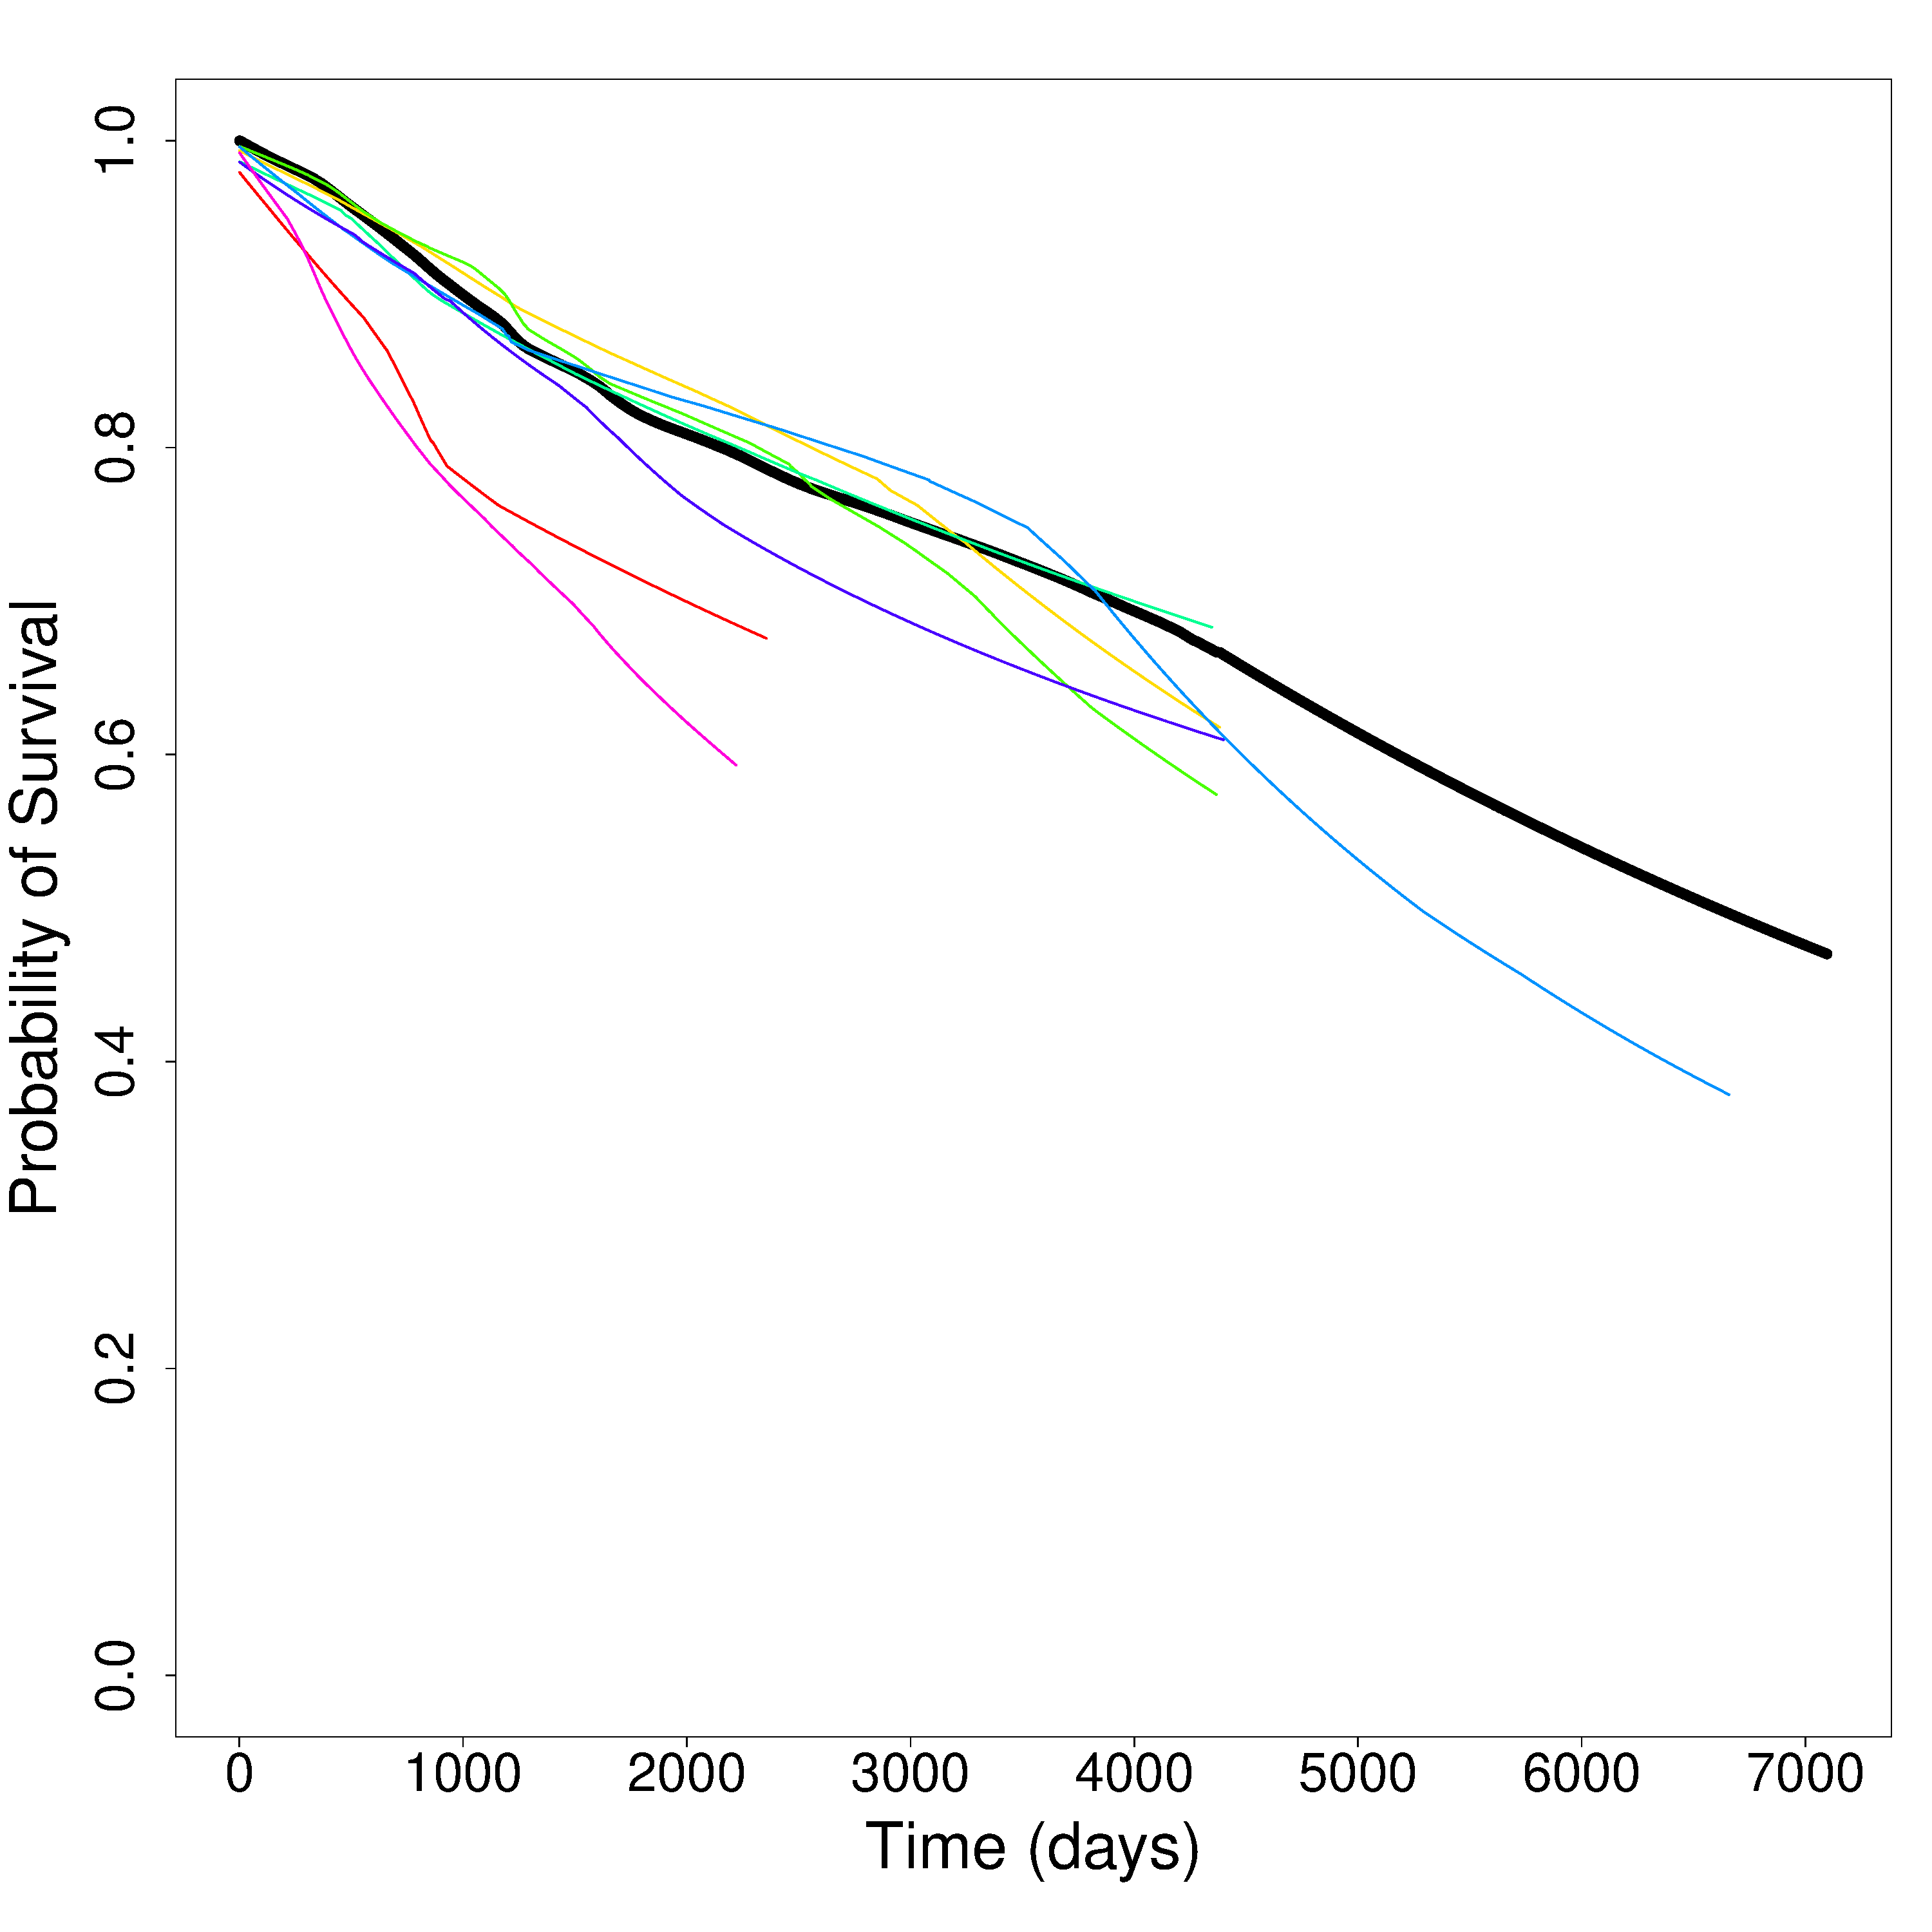
\includegraphics[width=7.5cm]{survival_plot.pdf}\\
  \caption{\textbf{Average probability of survival of each set and the
      combination of all sets for breast cancer}. The true models are different in true
    baseline cumulative hazard and coefficients. We can compute %the
    %average linear predictor and the survival function calculated with
    %the true cumulative hazard and the mean linear predictor. 
    a survival function for each individual in every dataset with the
    true cumulative hazard and the linear predictor. 
    We then average these survival functions across patients within each dataset.
    Colored lines represent average survival functions in each original
    sets, while the black, bold line shows the average survival function of
    all sets combined, with which we will later obtain the same true
    model in the simulation.}\label{survplot}
\end{figure}

%Figure \ref{scheme} summarizes the the methods and results of our
%study. We implemented the \emph{simulatorZ} Bioconductor package to
%simulate a collection of independent microarray studies based on
%experimental and clinical data, but with known ``true models''
%associating gene expression and clinical predictors to
%disease and metastasis-free survival.  

%Figure \ref{scheme} summarizes the methods and results of our
%study. 
In original and simulated data we observed
dramatic loss of survival discrimination accuracy, reductions of
approximately 0.04 on the C-index scale. We manipulated aspects of
the simulated data to establish that reducing heterogeneity in
prevalence of important clinical covariates and in gene expression
measurements were not sufficient to eliminate the loss of cross-study
prediction accuracy relative to within-study accuracy.  %Only enforcing
%identical ``true models'' of survival as predicted by gene expression
%was sufficient to eliminate the between to within-study gap in
%prediction accuracy.
Enforcing identical ``true models'' of survival as predicted by gene expression and clinical covariates
was sufficient to largely reduce and even eliminate the between to within-study gap in
prediction accuracy. %for breast cancer, but not in the ovarian cancer data.


  \subsection{Simulation Studies}

  We re-capitulated the major properties of %a compendium of 7
  %microarray studies of ER-positive breast cancer with censored
  %disease and metastasis-free survival (DMFS) outcome, 
  two collections of cancer microarray studies in a 3-step bootstrap
  simulation procedure. The effects of between-study heterogeneity
  were simulated by resampling of studies, and distribution and
  covariance of gene expression was preserved through resampling of
  individual patients within studies.  Linear models associating
  clinical/pathological variables and gene expression to outcome, as
  well as baseline survival functions and censoring distributions,
  were generated based on the original experimental data.  We
  emphasize that standard clinical factors were included as required,
  unpenalized covariates in the ``true'' prognostic model so that
  their associations with outcome would be guaranteed to be preserved
  across simulations. 
  These clinical covariates were also included as binary predictors along with
  gene expressions in the within and across-study validation.   

  The simulation resulted in within and across-dataset
  training/ validation characteristics comparable to those from prior
  clinical studies (Supplementary Figure 3).  Most importantly, the
  simulation studies maintained a marked difference in prognostic
  validation accuracy as estimated within studies and across studies
  by the C-index. This difference is seen for for Ridge regression 
  and the M\'{a}s-o-menos method, in breast cancer and ovarian cancer, 
  see panels "baseline" in Figure \ref{boxplot_breast_masomenos} and Supplementary Figure 1.



  \subsection{Eliminating Heterogeneity in Clinical Factors}

%  \begin{figure*}[!t]
%      \centering
%        \includegraphics[width=17cm]{boxplot-remove-d.pdf}\\
%    \caption{\textbf{Comparison of the C-index as assessed by cross
%      validation (CV) and cross-study validation (CSV) in 4 simulation
%      scenarios} labeled a, b,c and d.
%      Panel (a) is a baseline scenario not considering any source of
%      heterogeneity, showing better apparent prediction accuracy by
%      CV than by CSV.
%      In panel (b) bootstrap sampling probabilities are
%      re-weighted to equalize the distribution of
%      covariates in each study.
%      Panel (c) equalizes expression covariance structures by building true
%      models using only genes with high Integrative Correlation, which
%      impacts the performance of both CSV and CV. Neither (b) nor (c)
%      explains the decline of CSV performance.
%      %Panel (d) uses the same
%      %generative model for all datasets, \textit{i.e.}, the same linear risk
%      %score coefficients and the same baseline hazard, without equalizing
%      %covariate prevalence or covariance structure.  Prediction
%      %accuracy of CSV is brought up to the same level as CV.
%      %Panel (e) simulations equalize the baseline hazard function across
%      %studies, but allow different
%      %coefficients of the linear risk score, and do not equalize the
%      %CSV-CV difference.
%      In panel (d) the covariates distribution,
%      gene expression covariance are both manipulated. Also, the true generative models are
%      equalized, resulting in an apparent reduction in the difference between CSV and CV
%      performance . We can observe from this figure that
%      differences in gene / outcome association have the major role in
%      explaining the CV - CSV difference. This
%      figure is our major result, showing that for microarray-based
%      prediction of prognosis for ER-positive breast cancer,
%      equalizing the distributions of known prognostic factors and of
%      gene expression covariance across studies do not eliminate or
%      even reduce the diminishment of discrimination accuracy across
%      studies.}
%    \label{boxplots}
%  \end{figure*}

  To establish whether eliminating heterogeneity in known clinical
  factors could improve cross-study validation accuracy, we
  re-weighted bootstrap sampling probabilities to balance tumor size,
  grade and patient age for the breast cancer data, and age and 
  debulking status for the ovarian cancer data. Proportions of these factors
  were then the same, on average, for each simulated dataset. We observed that
  %that balancing these covariates improves the
  %performance of CV while worsening CSV, making the difference even
  %greater 
  balancing these covariates improves the performances of both CV and CSV for breast cancer. 
  For both cancer types, the differences between CV and CSV are not eliminated 
  (Figure \ref{boxplot_breast_masomenos} and Supplementary Figure 1, "rebalanced covariates"). In this scenario, differing distributions of these
  covariates across datasets does not contribute to the loss of
  prediction accuracy across studies relative to within studies.

  \subsubsection{Balancing the prevalence of clinical factors shuffles the rank of CSV scores}
  Though the prevalence of covariates does not account for the drop in accuracy in cross-study
  validation, we found that the rank of CSV scores is strongly affected. In other words, 
  the performance in individual cross-study training / test dataset pairs 
  is affected, with no overall effect across all training/testing pairs 
  (Supplementary Figure 5). To quantify this observation,
  we used a linear model for every covariate which associates the changes in proportions of 
  clinical factors to the changes in the CSV scores. We found that changing prevalence of  
  certain covariates, such as age and debulking status for ovarian cancer, does not significantly relate
  to the prediction accuracy changes, even when these covariates themselves are prognostic to the survival outcome (Table \ref{regress-table}).
  
  	
%  \subsubsection{Eliminating Heterogeneity in Prevalence of PGR Expressing Breast Tumors}
%  PGR was available in only 5 datasets in the breast cancer studies, so we balanced it separately
%  from the other clinical covariates.  Using only these 5 datasets for
%  both the baseline and balanced scenario, the difference between CV
%  and CSV was again not improved (Supplemental Figure 5).

 
  \subsection{Filtering Genes by Integrative Correlation}
  %To mitigate the potential for degradation of cross-study validation
  %by batch effects or platform effects, we used only genes
  %Integrative Correlation \citep{Parmigiani2004, Garrett-Mayer2008} greater than 0.4
  %between all pairs of studies. This reduced the number of genes from
  We searched on grid for the threshold of Integrative Correlation \citep{Parmigiani2004, Garrett-Mayer2008} to include roughly the top 1000 genes with the highest Integrative Correlation between every pair of original datasets. The threshold is 0.24 for breast cancer (999 genes), and 0.15 for ovarian cancer (1002 genes). After filtering these genes on the original datasets, the variance of C-statistics across simulations increases, but the differences between CV and CSV are not equalized. 
  
  As a comparison to grid search, we used arbitrary thresholds of 0.4 for breast cancer and 0.2 for ovarian cancer. Using only genes with Integrative Correlation greater than 0.4 reduced the number of genes from 5307 to 343 (6.5\%) for breast cancer. A threshold of 0.2 reduced the number of genes 
  from 7484 to 590 (7.9\%) in ovarian cancer data. Both CV and CSV performs slightly worse using the fixed thresholds compared to the grid search, which results from the loss of good predictors due to strict filtering. The observed pattern remains (Supplementary Figure 6), which suggest that the result is robust to the two choices of thresholds. Filtering genes to enforce similar
  covariance structures across studies, as would be expected in the
  absence of microarray batch or platform effects, also does not
  remove the CV-CSV difference.
  
%  Both CV and CSV performance are similarly slightly reduced by this reduction in
%  available predictors. The variance of C-statistics across
%  simulations also increases. Filtering genes to enforce similar
%  covariance structures across studies, as would be expected in the
%  absence of microarray batch or platform effects, also does not
%  mitigate the CV-CSV difference.

  \subsection{Using the Same True Model}

  True models of experimental sets differ in both baseline survival and
  coefficients. Figure \ref{survplot} shows the average probability of
  survival in each dataset and for all datasets combined. Differences
  in baseline survival mean that survival across all patients is better in some
  datasets than others, for example varying between 60\% and nearly 90\% 5-year
  survival. We equalized both coefficients and baseline hazards across studies.

  Utilizing true survival models that are identical in both
  baseline survival and coefficients is sufficient to eliminate the
  difference between within and across-study validation for breast cancer
  (Figure \ref{boxplot_breast_masomenos} and Supplementary Figure 1, "same models"), whereas
  equalizing only the baseline survival functions has negligible effect
  (Figure \ref{boxplot_breast_masomenos} and Supplementary Figure 1, "same hazard").   
  
  Enforcing the identical true models does not completely erase the differences between CV
  and CSV for the ovarian cancer data, but the differences are greatly reduced 
  compared to baseline simulation.
  
  %Equalizing the true models over and above equalizing clinical and
	%pathological covariates and gene covariance provides the most
	%substantial reduction in the gap between average prediction scores of
	%CV and CSV. The equalization between CV and CSV seen in panel (d)
	%relative to the other panels in the boxplots indicates
	%substantial differences in the association between predictors and the
	%survival response are responsible for the most important degradation
	%in CSV scores.
   

  %possibly related to the observation of a 
  %less consistent covariance structure in the ovarian cancer database (section 3.3).

  \subsection{Combination of three factors}
  %We also evaluated the effect of equalizing all three types of
  %heterogeneity (Figure \ref{boxplots}f).  The gap
  %reduces to approximately 0.01 or 0.02. Also, the effects in panel(d)
  %and (f) look very much alike. \fixme{In the version I see, CV and
    %CSV are essentially identical in (d), but CV is better by about
    %0.02 in (f).  Equalizing true models only does a better job of
    %equalizing the CV/CSV difference than equalizing all sources of
    %heterogeneity?  Just want to make sure this is right, it's a bit
    %hard to explain.}

    %Combining the two sources we inspected with simulations, while using identical
%Equalizing the true models over and above equalizing clinical and
%pathological covariates and gene covariance provides the most
%substantial reduction in the gap between average prediction scores of
%CV and CSV. The equalization between CV and CSV seen in panel (d)
%relative to the other panels in the boxplots indicates
%substantial differences in the association between predictors and the
%survival response are responsible for the most important degradation
%in CSV scores.

	When using identical models, balancing the clinical factors
	and selecting genes with high Integrative Correlation at the same time, 
	we found that the combined alteration almost removes the CV-CSV differences. 
	A small gap was re-introduced in between the averaged CV and CSV scores 
	compared to using only identical true models which equalizes them 
	(Figure \ref{boxplot_breast_masomenos} and Supplementary Figure 1, "all of the above"). However this difference is much smaller than	baseline. 
	%This 
	%shows again the effect of clinical factors in 
	%slightly enhancing the differences of prediction accuracy between 
	%cross-study validation and conventional CV. 
	

  \subsection{Eliminating Outlier Datasets}
  Supplementary Figure 3 identifies the CAL dataset as an outlier with
  much greater difference between cross-validation and cross-study
  validation than other breast cancer datasets in simulation, and with C-indices of
  approximately 0.48 when it is used for training, validation, or
  cross-validation in original experimental data.  To establish the
  impact of this outlier dataset, we repeated all simulations with it
  removed (Supplementary Figure 8). %Results under every condition follow the same trends as
  %illustrated above (Supplemental Figure 7).

  Removal of CAL improves the performances of both CV and CSV. CSV is more affected by this outlier dataset. We observed that CSV performances increase to a greater extent compared to the CV performances in all simulations except for the one where identical true models are used. Thus the
  prediction accuracy drop is mitigated for the rest of the simulations. However, results under 
  every condition still follow the same trends as illustrated above.
  
\section{Discussion}

It is commonly assumed that heterogeneity in experimental platforms or
procedures, and differences in patient cohorts, compromise the
comparability of independent datasets and the application of
omics-based prediction models across studies.  The obvious solution is
to minimize potential sources of heterogeneity, for example by
enforcing precise inclusion criteria for patient inclusion in clinical
studies.  However, such narrowing has costs in sample size and
potential generalizability of findings.  To the best of our knowledge,
no study has suggested a systematic approach to assessing the impact
of suspected sources of heterogeneity on across-study performance of
prediction models.

When training and validating microarray-based survival models in two 
compendia consisting of 7 breast cancer datasets and 5 ovarian cancer datasets,  
%estrogen-receptor positive breast cancer studies, we
we observed a discrepancy in C-index for models validated in fully
independent studies when compared to standard cross-validation.
Independent validation statistics were 0.04 worse on the
C-index scale for independent validation when compared to
cross-validation, a sizeable difference that could yield
cross-validation almost meaningless for deciding whether to pursue
follow-up experiments for a prediction model developed and validated
on only a single dataset. We thus investigated the contributions of
known and unknown sources of heterogeneity to this discrepancy.

In simulations mimicking these two compendia of datasets, decreasing
heterogeneity in important clinical covariates %(patient
%age, tumor size and grade, and PGR status) 
did not reduce the
discrepancy between CV and CSV. %; rather it enhanced  CV and increased
%the discrepancy. This surprising finding has several likely
%explanations. % Patient age dichotomized at 50 was not observed to be a
% prognostic factor, consistent with the literature.  Therefore unless
% gene expression profiles are systematically different for younger and
% older patients, reducing age differences would not be expected to
% improve cross-study validation.
%Several covariates are expected to be associated with
%both gene expression profiles and survival, such as tumor size and grade for breast cancer. 
%If the prognostic value
%of these factors is sufficiently redundant to gene expression, then
%shifts in their prevalences would not impact on prognostic model
%accuracy across studies. However, more mixing of prognostic clinical
%and pathological covariates within studies, as occurs when balancing
%them between studies, makes within-study prediction ``easier''.  
This finding highlights that it should not be assumed that known
differences in the composition of different cohorts will negatively
impact the application of prediction models across them, or that
stricter inclusion criteria will improve the models.

% It is likely that after balancing clinical covariates, the prediction
% improves in cross validation, especially when the original data set is
% biased in a certain level of the covariate. But in cross-study validation,
% it is likely that a repetition of gene expressions in the simulated data sets
% results in a slight decrease in the performance.
%Also, there could be genes
%that correlate with the covariates in one set but do not in others,
%which impedes an increase in the CSV scores.

Mixed-effect models were used to associate the changes 
in proportions of clinical covariates to the accuracy
degradation across studies. %All interaction terms 
%are positive in these models, regardless of whether main effects 
%are positive or negative. So to the limited extent that matters, consistency in 
%train/test covariate prevalence is better for prediction.
%The negative estimates for debulking in both train and 
%test for ovarian cancer suggest that survival for 
%optimally debulked tumors is not predictable and 
%these tumors do not help in building survival models, 
%although the positive interaction term still suggests a 
%benefit of consistency in prevalence of optimal debulking.
Interestingly, we found that although some covariates strongly affect survival, 
they do not have much impact on the prediction of survival. Heterogeneity in the prevalence 
of covariates like debulking and patient age for ovarian cancer can impact 
overall survival, but not the ability to predict overall survival.

Similarly, in these compendia of datasets spanning at least 11 different labs
and 4 different microarray technologies, enforcing good
expression measurement comparability through selection of genes with
high Integrative Correlation \citep{Parmigiani2004, Garrett-Mayer2008} did not improve
the comparability of cross-study validation and cross-validation. Only
ensuring fully identical models of association between gene expression
and outcome for each study was sufficient to eliminate this
discrepancy. %for the breast cancer type.  
We liken this heavy-handed approach to study equality to
correcting for the impacts of all possible unknown sources of
between-study heterogeneity. Thus in these datasets, the most
important sources of heterogeneity from the perspective of cross-study
validation are not recorded in the published datasets.

This study has several limitations. %We performed simulations only in
%the context of ER-positive breast cancer , because the capability for
%developing accurate prognostic models is good enough that the
%constrast between cross-study validation and cross-validation is
%stark.  
%Our findings are disease context-specific, but our proposed
%approach shows how the impact of known sources of study heterogeneity
%can be assessed for their impact on prediction modeling, and that the
%most obvious heterogeneity may not be the most important. We focused
%on only one prediction algorithm \citep{Zhao2014}, chosen for its
%speed and previously demonstrated good performance in these datasets
%\citep{Bernau2014}. 
We performed simulations only in the context of ER-positive breast cancer and
late-stage, high-grade ovarian cancer, using only two prediction algorithms. But our proposed
approach shows how the impact of known sources of study heterogeneity
can be assessed for their impact on prediction modeling, and that the
most obvious heterogeneity may not be the most important. 
We could only analyze clinical
heterogeneity that was available in sufficient numbers of these
datasets: patient age, tumor size and grade for breast cancer;
age and debulking status for ovarian cancer.  By
publishing the \emph{simulatorZ} Bioconductor package, which automates
all steps of these simulations including covariate balancing, as well
as a code repository to reproduce the results of this paper, we hope
to encourage further investigation of the effects of study
heterogeneity in other predictive modeling contexts.

% We used package which combines functions for the simulation of
% independent genomic datasets and using predicting modeling to generate
% a summarization matrix of C statistics, to evaluate possible causes
% for the decrease of the predicting score performances in cross study
% validation. The three potential causes of this phenomenon behave
% differently in our simulations: 1). Covariate shift will improve the
% performance of cross validation and enhance the difference between
% cross validation and cross-study validation; 2). Using features that
% varies in similar magnitude across studies will improve both
% prediction accuracy as well, but in a slighter degree than covariate
% shift does. It does not account for the difference between them; and
% 3). The same true models used for simulating datasets will reduce the
% gap significantly.

% Our study provides both software tools for more similar
% implementation, and inspiring results that can help the development of
% using prognostic models in clinical problems. The package, which,
% although derived from fitting our needs in the simulations,
% became more flexible for multiple classes of data
% sets. It has the potential for handful use under multiple
% settings.

% The results suggest that covariates shift in population
% and microarray platform effect may not be the source of degraded CSV
% performance, while study-specific associations between gene expression
% and outcome are primarily responsible for it. The framework of our simulation
% is based on the concept that finite populations of interest can be viewed as
% samples from an infinite "super-population" \citep{Hartley1975-bj}. Results
% show that models tends to over-estimate prediction accuracy in ER+ breast
% cancer relative to independent datasets, for study-specific reasons
% unrelated to covariate shift. Similarly, platform effect can be ruled out
% by filtering for gene covariance as well. After we witnessed the change
% made by using the same true model, we separated the model into coefficients and
% cumulative hazards, then we saw the CSV degraded again when using the same hazards
% but different coefficients. We can conclude from it, that the
% specific associations between gene expression and response
% account for the decline of CSV validation accuracy.

% We can also conclude that even independent validation does not
% eliminate the risk of over-optimism without comparative
% evaluation. The importance of direct comparative evaluation of newly
% proposed gene signatures against existing signatures or random
% signatures has already been addressed, e.g. evaluation of Dressman et
% al. datasets in \citet{Waldron2014}. Independent, comparative
% validation should be the gold standard evaluation of genomic
% prediction models.



\section{Acknowledgement}

This work was supported by grants from the National Cancer Institute
at the National Institutes of Health (1RC4CA156551-01 and 5R01CA142832
to GP, and 5R03CA191447-02 to LW).


\bibliographystyle{natbib}
\bibliography{bibfile}

\end{document}

% From Christoph
% possible reason for difference in figure 3 panel a->c
% ----------------------------------------------------------


% CV goes up becomes after balancing for covariates, good C-indices
% can be achieved by simply predicting the clinical covariate
% (e.g. which is clearly predictive for survival) from the gene
% expressions

% if the original dataset been very homogeneous with regard to the
% covariates prediction on the original data set has been much harder
% because you cannot achieve good results by recovering information
% about the clinical covariates from the gene expressions. Only truely
% new information (c.f. additional predictive value n the literature)
% from the gene expresisons can used for discriminating beween the
% patients and we know that this is much harder (additional predictive
% value has been often found to be modest in earlier papers).



% But why don't we see this effect for CSV?

% This could be something like the surrogate genes, we have discussed
% earlier?

% what if there are some genes which are only correlated to the
% clinical covariates on certain data sets but not on the others ? In
% this case, i.e. if those genes get assigned high coefficients by
% plsuminus although they are just spuriously correlated and on
% another study we will get poor results using this prediction rule
% (indeed, if this theory holds, the whole effect should be less
% pronounced if only genes with high integrative covariance are used).
% The 'advantage' the algorithm has in CV is that it simply does not
% matter whether it finds spuriously (on this specific data set)
% correlated or truly correlated genes. prediction performance will
% not be reduced.

% By the way, ballancing the clinical covariates also increases the
% 'signal' in the data (if the original data set has been clinically
% homogeneous) which should increase the probability of higher
% coefficients (or in the case of plusminus, maybe more non-zero
% coefficients) which should lead to more variance in the linear
% predictor which could explain the larger variance of the c-index in
% panel c (though we also have to see that this increase in variance
% does not exist ).


% UNT
% ----

% in the new paper we have a strong counter-intuitive pattern for UNT
% on the original data set (C-Index in CSV clearly higher than in CV)
% which is reversed on the simulated data.

% a similar pattern though less pronounced exists in the ZRanking
% paper for ridge and some other algorithms. However, e.g. for Lasso
% it is just the other way around, i.e. the pattern is not consistent
% over the algorithms.

% It could be related UNT being a small data set (70obs) and the
% conjuncture that plsuminus and ridge seem to have a flatter learning
% cave (i.e. needs more observations 'before it believes that it has
% found an existing pattern/signal' in the data) which also seems to
% make those algorithms less prone to overfitting which seems to be
% better for archieving good CSV results.
